\newcommand{\hl}[1]{\colorbox{yellow}{#1}}

\chapter{Vorlesung 9}
\section{Vergleichbasierte Sortieralgorithmen}

\pagebreak

\section{Radix-Sort}

\subsection{Beispiel:}
\begin{tabular}{l l l l}
  10\hl{1} & 0\hl{1}0 & \hl{1}00 & 001 \\
  01\hl{0} & 1\hl{0}0 & \hl{1}01 & 010\\
  00\hl{1} & 1\hl{1}0 & \hl{0}01 & 011 \\
  11\hl{1} & 1\hl{0}1 & \hl{0}10 & 100 \\
  10\hl{0} & 0\hl{0}1 & \hl{1}10 & 101 \\
  01\hl{1} & 1\hl{1}1 & \hl{1}11 & 110 \\
  11\hl{0} & 0\hl{1}1 & \hl{0}11 & 111 \\
\end{tabular}
\paragraph{Wichtig}Beginne die Sortierung mit dem niedrigsten Bit

\subsection{Pseudo-Code}
\lstinputlisting[language=Java]{9/Code/radixsort.java}


\pagebreak

\section{Binäre Suchbäume}

\paragraph{Zahlen} 12, 8, 3, 16, 24, 17, 10, 21, 14, 9 

\begin{figure}[H]
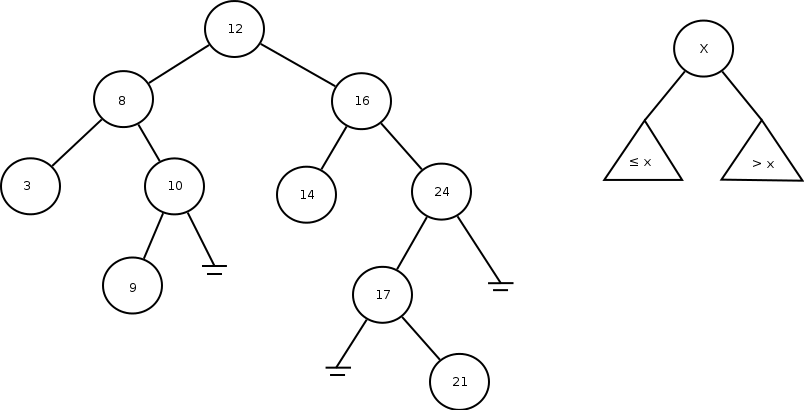
\includegraphics[width=\linewidth]{9/Grafik/img4.png}
\captionsetup{justification=raggedright, singlelinecheck=false}
\caption{Knotenorientierte Speicherung}
\end{figure}
